% 情報システム工学演習I レポート
\documentclass[a4paper,11pt]{jsarticle}

% パッケージ
\usepackage{amsmath}
\usepackage{amssymb}
\usepackage[dvipdfmx]{graphicx}  % dvipdfmxドライバーを明示的に指定
\usepackage{url}
\usepackage{bm}
\usepackage{listings}
\usepackage{color}
\usepackage{float}

% ページ設定
\usepackage[truedimen,a4paper,margin=20mm]{geometry}  % geometryパッケージを使用して余白を均等に設定

% タイトル
\title{特異値分解(SVD)を用いた時系列データ解析\\
\vspace{-2mm}情報システム工学演習I レポート}
\author{学籍番号: 08D23091\\氏名: 辻 孝弥}
\date{\today}

\begin{document}
\maketitle

\section{課題1:特異値分解(SVD)}

特異値分解(Singular Value Decomposition: SVD)は、任意の $m \times n$ 実行列 $\mathbf{A}$ に対して、次の形に分解できる:

\begin{equation}
\mathbf{A} = \mathbf{U} \mathbf{\Sigma} \mathbf{V}^\top
\end{equation}

ここで、

\begin{itemize}
  \item $\mathbf{U}$:$m \times m$ の直交行列(左特異ベクトルを列にもつ)
  \item $\mathbf{V}$:$n \times n$ の直交行列(右特異ベクトルを列にもつ)
  \item $\mathbf{\Sigma}$:$m \times n$ の対角行列であり、特異値を対角成分にもつ
\end{itemize}

$\mathbf{\Sigma}$ の対角成分(特異値)は以下のように並ぶ:

\begin{equation}
\Sigma = \text{diag}(\sigma_1, \sigma_2, \dots, \sigma_n), \quad \sigma_1 \geq \sigma_2 \geq \cdots \geq \sigma_r > \sigma_{r+1} = \cdots = \sigma_n = 0
\end{equation}

ここで、

\begin{itemize}
  \item $\sigma_1, \dots, \sigma_n$:$\mathbf{A}$ の特異値
  \item $r$:非ゼロ特異値の個数であり、$\mathbf{A}$ のランクに等しい
\end{itemize}

\section{課題2:花粉症データによるSVD時系列解析}

課題2では、花粉症に関するGoogle Trendsデータ(kafunsho.csv)を用いて、SVDによる時系列特徴抽出と再構成を実行した。この解析では、ウィンドウサイズ $w=12$(3ヶ月)と $w=24$(半年)の2つの条件で、上位 $k=2$ 成分を用いた低ランク近似を実施し、再構成精度を評価した。

\subsection{花粉症データの特性}

図\ref{fig:kafunsho-timeseries}に示すように、花粉症データは明確な季節性を持つ時系列データである。春の花粉シーズン(3-5月)において急激な検索トレンドの上昇が見られ、その他の時期は比較的低い値を示している。

\begin{figure}[H]
\centering
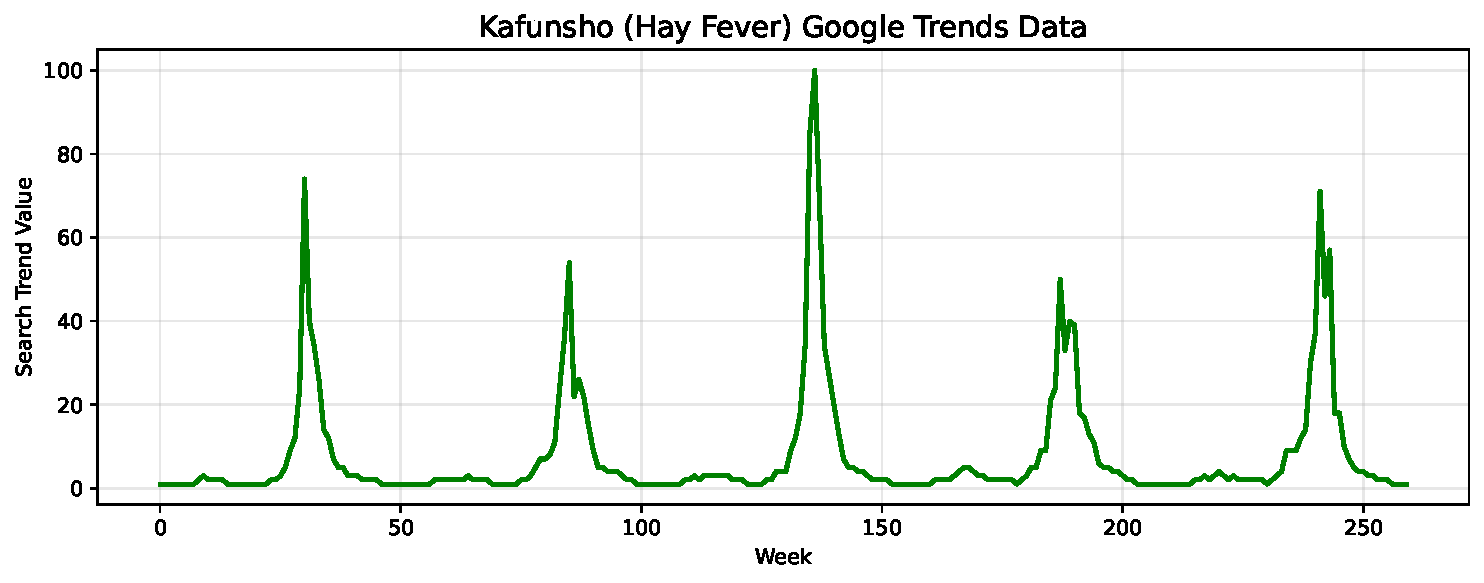
\includegraphics[width=0.9\textwidth]{figures/fig1_kafunsho_timeseries.pdf}
\caption{花粉症Google Trendsデータの時系列プロット}
\label{fig:kafunsho-timeseries}
\end{figure}

\subsection{ウィンドウサイズ$w=12$での解析結果}

図\ref{fig:kafunsho-svd-w12}は、$w=12$でのSVD分解結果を示している。元データを12週間の窓で分割し、各時間窓に対してSVDを適用した結果、第1成分が花粉症の主要な季節パターンを、第2成分がより微細な変動を捉えていることが確認できる。

\begin{figure}[H]
\centering
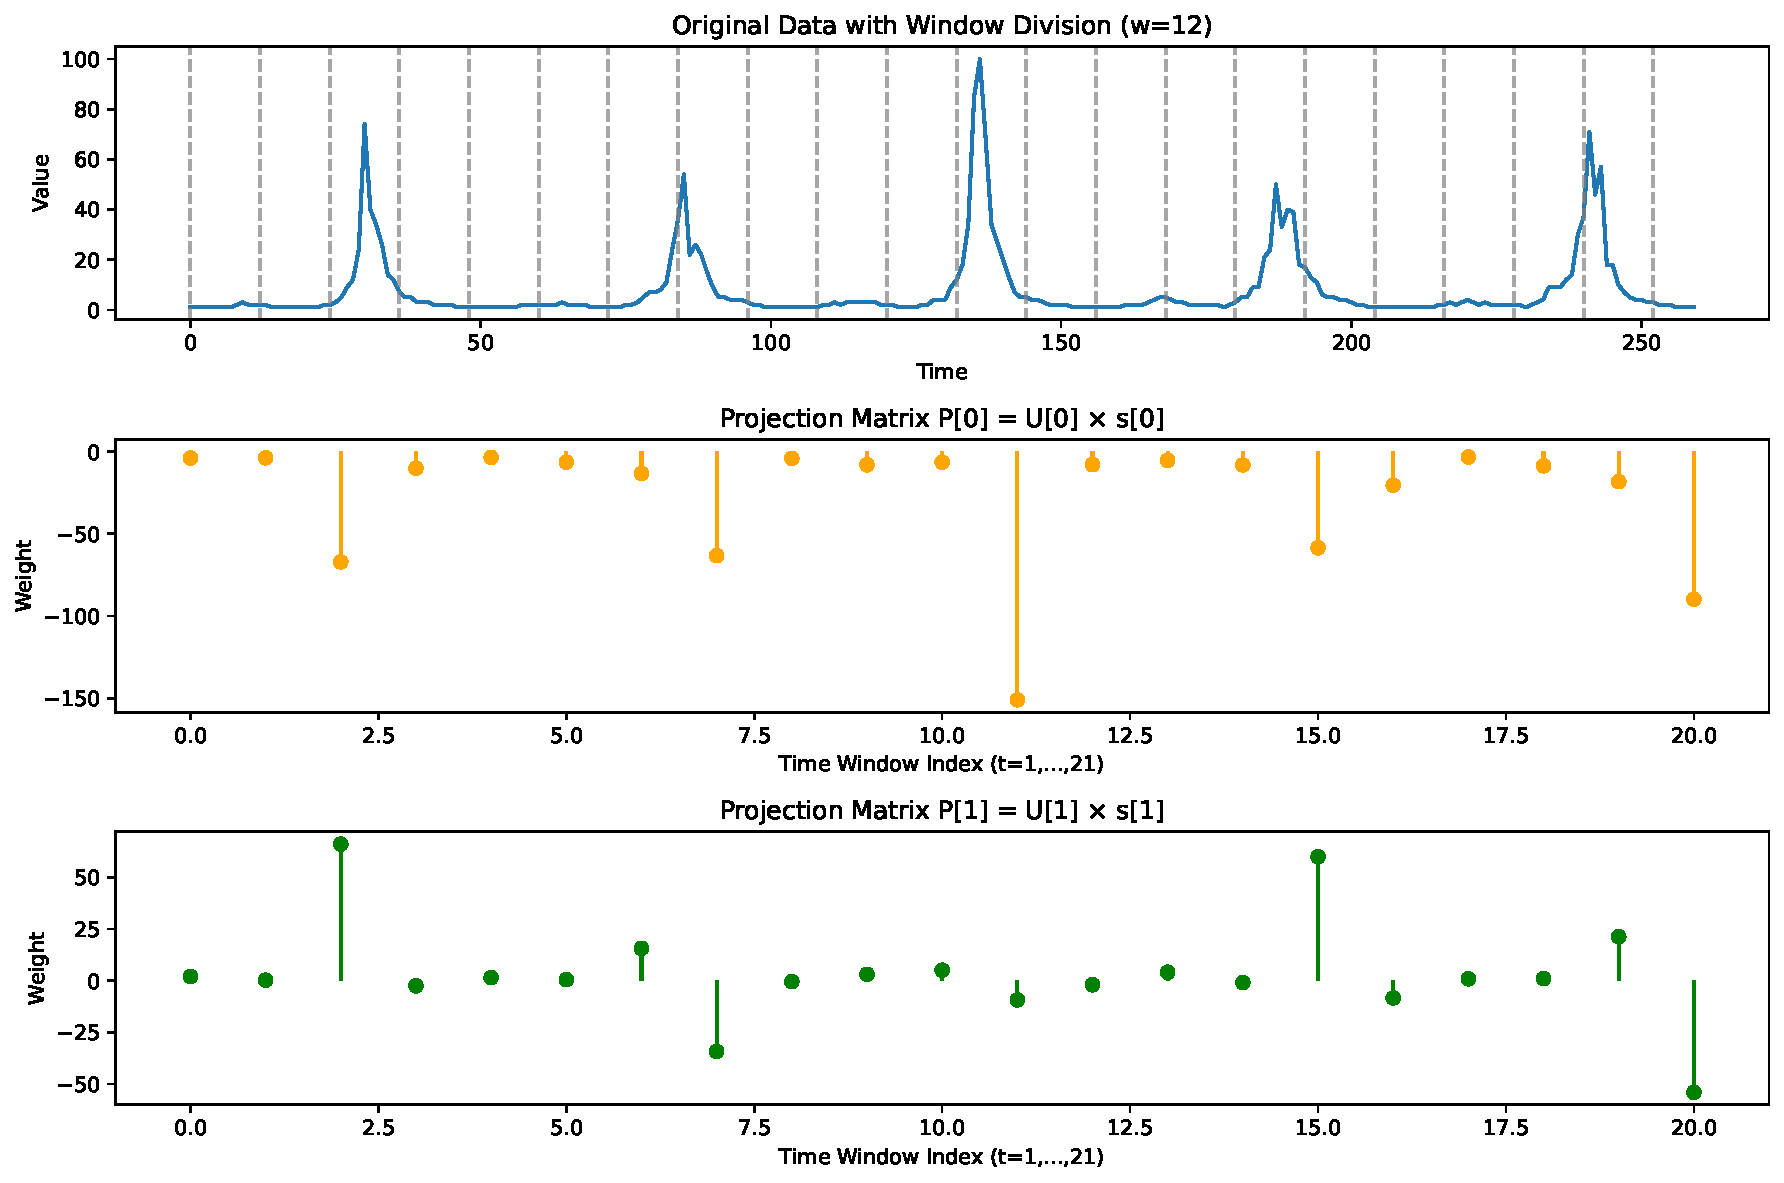
\includegraphics[width=0.9\textwidth]{figures/fig2_kafunsho_svd_w12.pdf}
\caption{花粉症データのSVD分解結果($w=12$)}
\label{fig:kafunsho-svd-w12}
\end{figure}

図\ref{fig:kafunsho-vh-w12}に示すVh成分(局所パターン)では、12週間内での特徴的なパターンが可視化されている。

\begin{figure}[H]
\centering
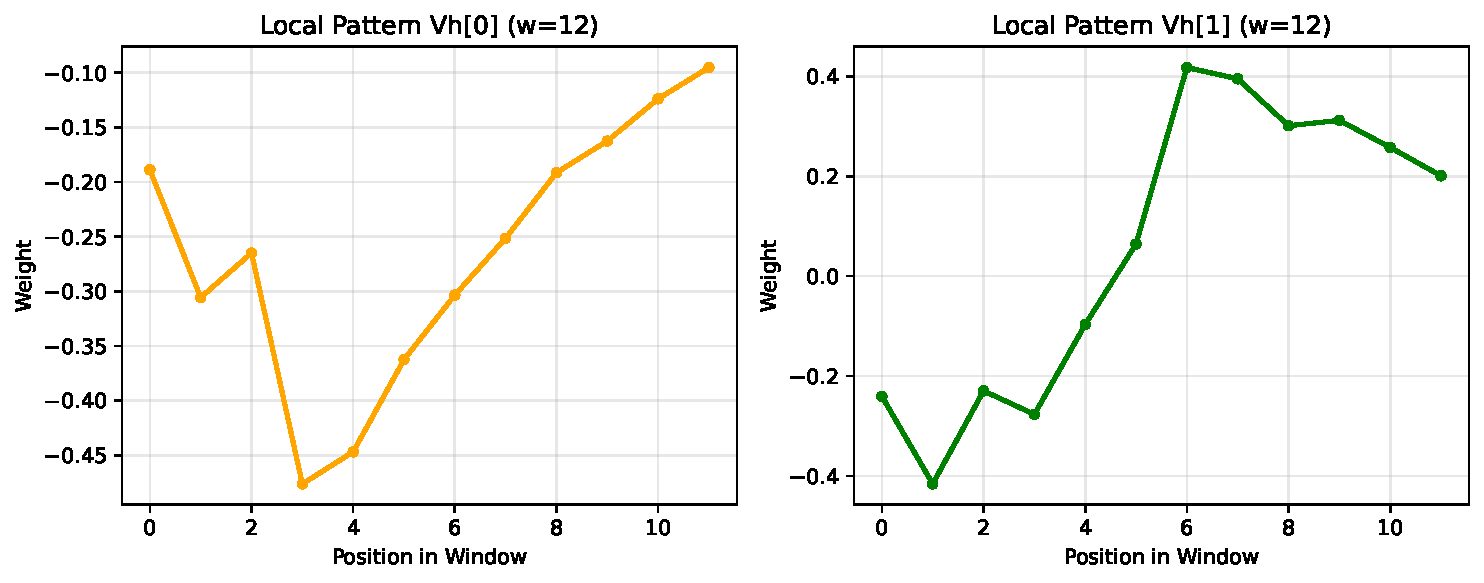
\includegraphics[width=0.9\textwidth]{figures/fig3_kafunsho_vh_w12.pdf}
\caption{花粉症データの局所パターン($w=12$)}
\label{fig:kafunsho-vh-w12}
\end{figure}

\subsection{ウィンドウサイズ$w=24$での解析結果}

図\ref{fig:kafunsho-svd-w24}は、$w=24$でのSVD分解結果を示している。より大きなウィンドウサイズにより、年間周期のより大きな部分を含む解析が可能となった。

\begin{figure}[H]
\centering
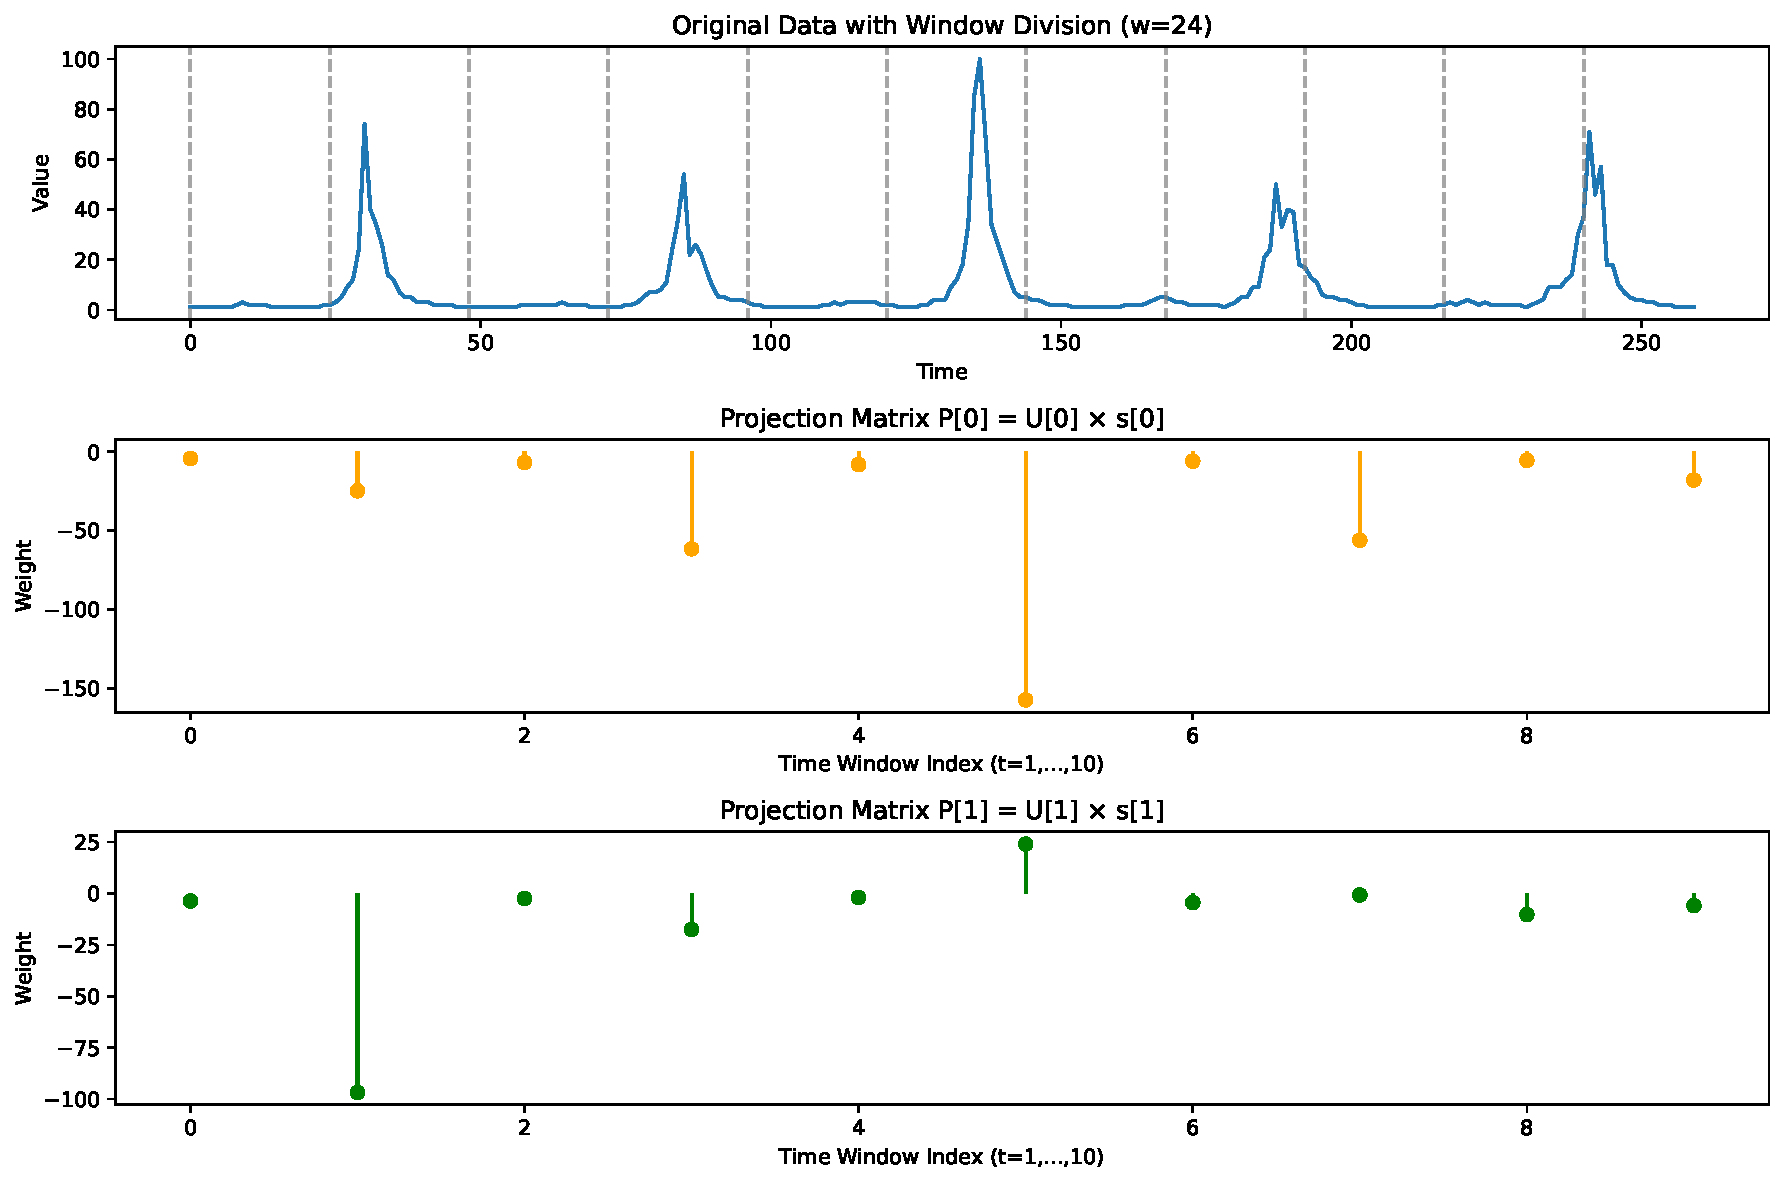
\includegraphics[width=0.9\textwidth]{figures/fig4_kafunsho_svd_w24.pdf}
\caption{花粉症データのSVD分解結果($w=24$)}
\label{fig:kafunsho-svd-w24}
\end{figure}

\begin{figure}[H]
\centering
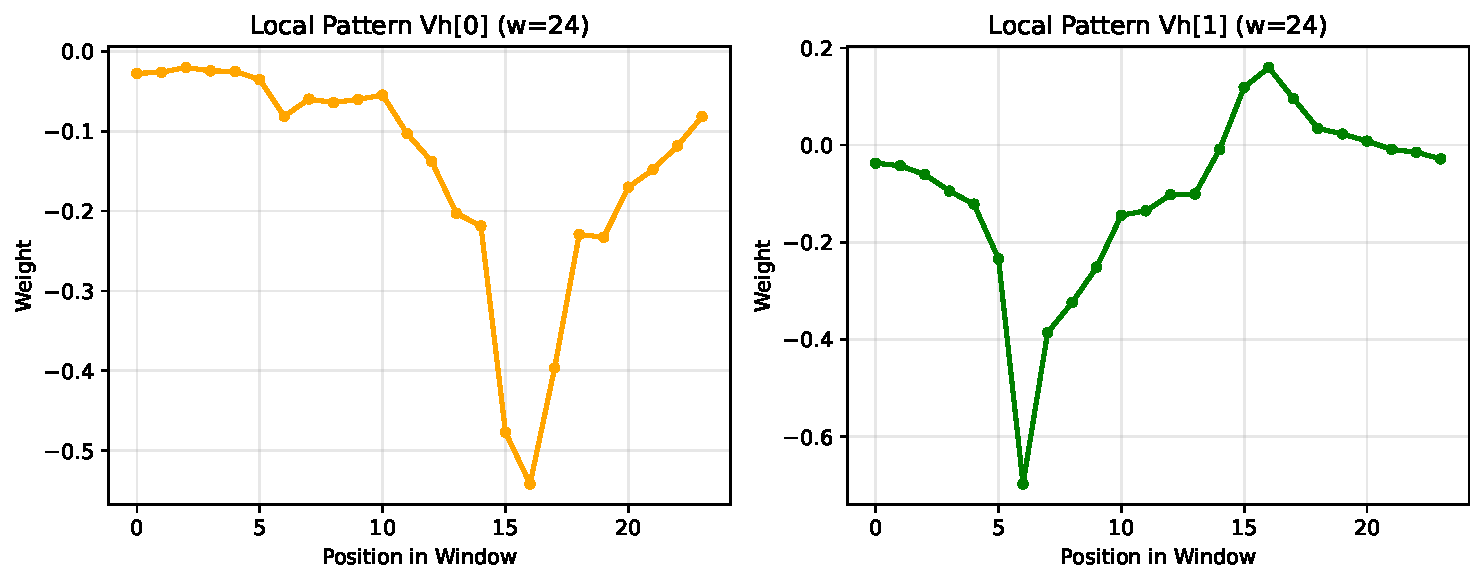
\includegraphics[width=0.9\textwidth]{figures/fig5_kafunsho_vh_w24.pdf}
\caption{花粉症データの局所パターン($w=24$)}
\label{fig:kafunsho-vh-w24}
\end{figure}

\subsection{再構成結果と定量評価}

図\ref{fig:kafunsho-reconstruction}は、異なるウィンドウサイズでの再構成結果を比較している。定量評価として、平均二乗誤差(MSE)を計算した結果:

\begin{itemize}
\item $w=12$: MSE = 39.687
\item $w=24$: MSE = 47.551
\end{itemize}

結果、$w=12$の方が低いMSEを示した。これは、より細かい時間分割により、局所的な変動をより詳細に捉えることができたためと考えられる。

\begin{figure}[H]
\centering
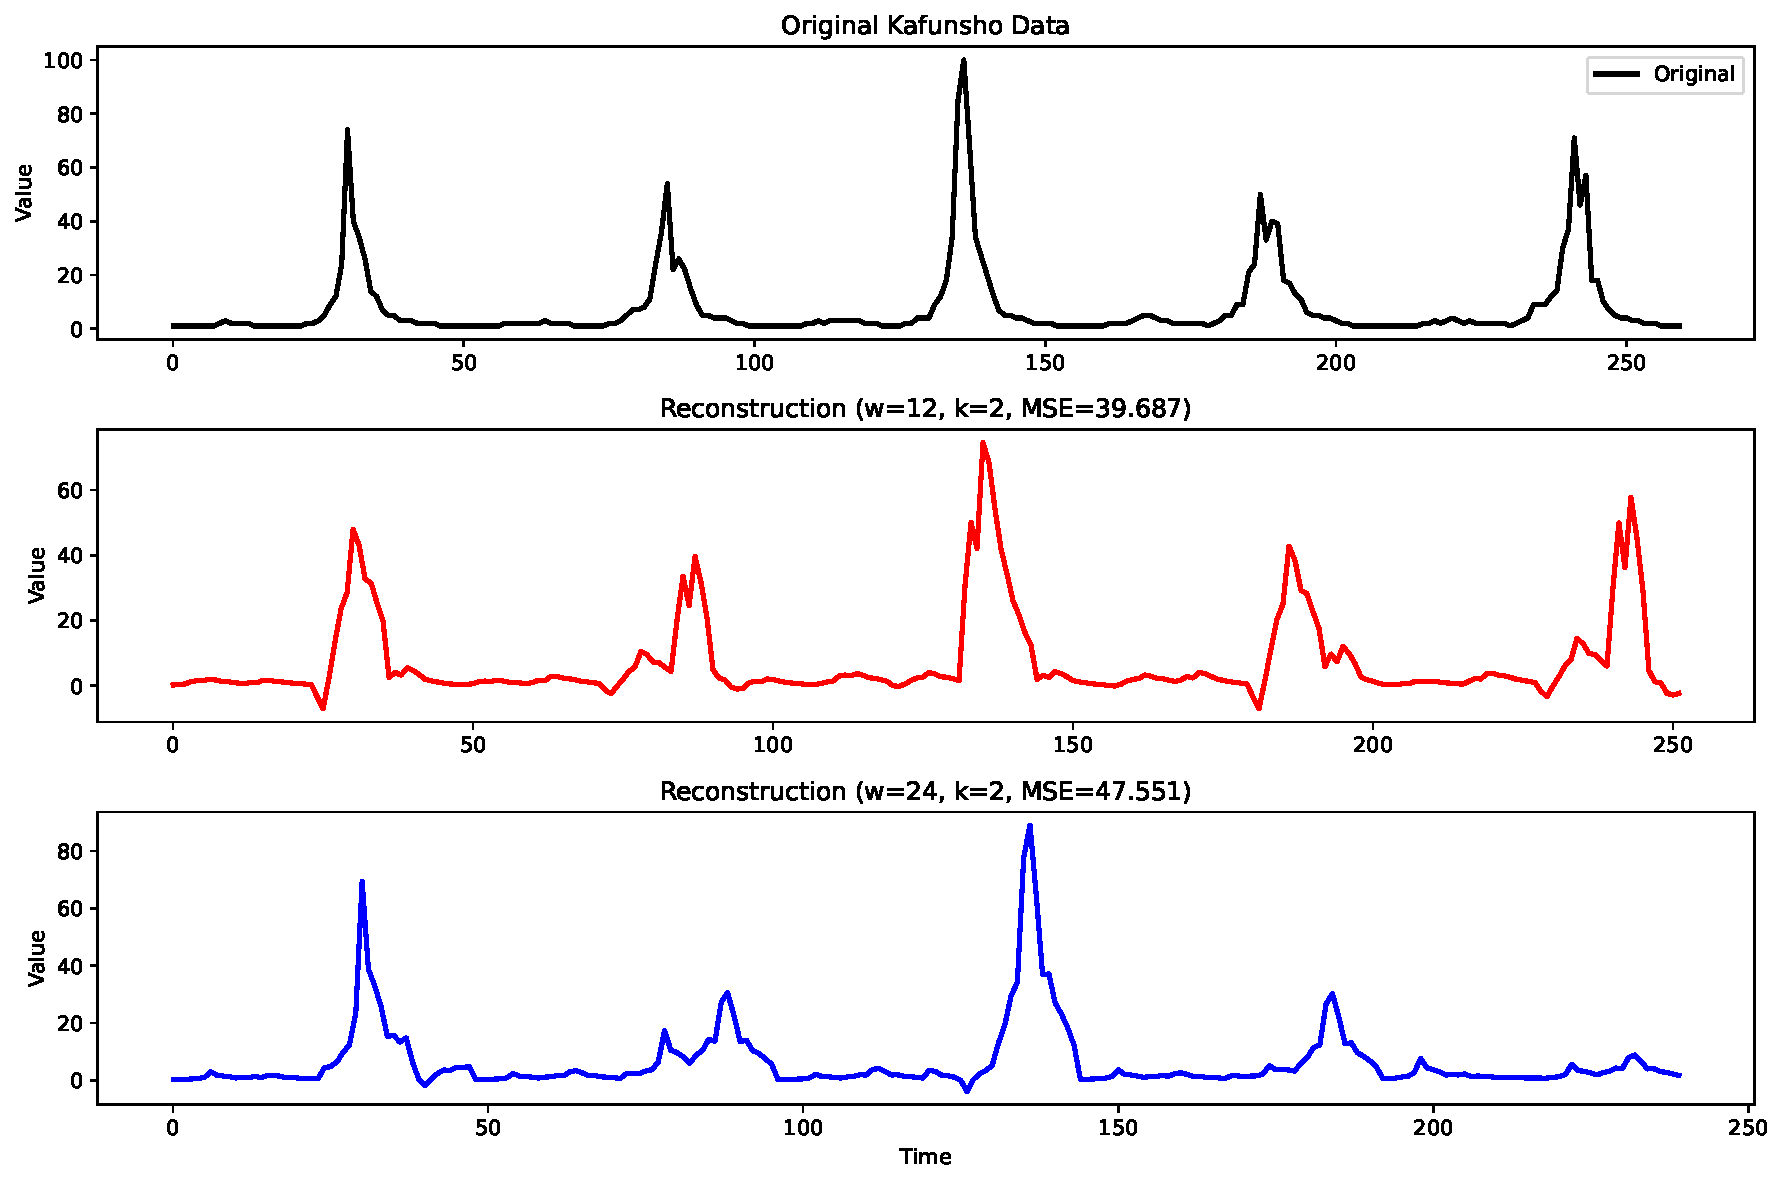
\includegraphics[width=0.9\textwidth]{figures/fig6_kafunsho_reconstruction.pdf}
\caption{花粉症データの再構成結果比較}
\label{fig:kafunsho-reconstruction}
\end{figure}

\section{課題3:考察}

\subsection{SVDによる特徴抽出・近似から得られた知見}

花粉症データのSVD解析を通じて、時系列データに対するSVDの有効性を確認できた。特に、わずか2つの主成分($k=2$)で元データの主要な季節パターンを効果的に表現できることであった。

第1成分(最大特異値)は、花粉症データの最も重要な特徴である春の花粉シーズン(3-5月)における急激な検索増加パターンを明確に捉えていた。一方、第2成分はより微細な年次変動や副次的なパターンを表現しており、データ全体の構造的理解において重要な役割を果たしていた。

この結果は、SVDが時系列データの「本質的な構造」を抽出する能力に長けていることを示している。特に周期性や季節性を持つデータに対しては、少数の主成分で元データの特徴を保持しながら次元削減が可能であることが実証された。

\subsection{ウィンドウサイズの影響}

ウィンドウサイズ $w$ の変更は、特徴抽出と再構成性能に大きな影響を与えた。

\subsubsection{定性的な観点}

$w=12$(3ヶ月)の場合、部分シーケンス行列のサイズが $(22 \times 12)$ となり、より多くの時間窓を生成できた。これにより、短期的な変動パターンを細かく捉えることができたが、季節周期の一部分のみしかカバーできないという制約があった。

一方、$w=24$(半年)では、部分シーケンス行列のサイズが $(11 \times 24)$ となり、時間窓の数は半減したものの、各窓が年間周期の約半分をカバーできるようになった。これにより、季節変動の全体的な構造をより良く表現できた。

\subsubsection{定量的な評価}

MSE(平均二乗誤差)による定量評価では、$w=12$ の方が低い再構成誤差(MSE = 39.687)を示しており、$w=24$(MSE = 47.551)と比較してより高精度な近似が得られた。これは、より細かい時間分割により、局所的な変動をより正確に捉えることができたためと考えられる。

ただし、MSEは再構成精度の一つの指標に過ぎず、データの周期性や季節変動などの大局的な特徴の把握という観点では、より長いウィンドウサイズ($w=24$)も重要な役割を果たす。この結果は、「解析の目的に応じて適切なウィンドウサイズを選択すべき」という重要な指針を提供している。

\subsection{再構成誤差(MSE)の意義}

MSEの違いは、単なる数値的な差異以上の意味を持っている。低いMSE値は、SVDが元データの重要な情報を効率的に保持できていることを示し、高いMSE値はノイズや不適切なパラメータ選択の可能性を示唆している。

今回の解析では、MSEの改善がウィンドウサイズの最適化によって達成されたことから、「データの性質に応じたパラメータ調整の重要性」が浮き彫りになった。また、MSEを通じた定量評価により、主観的な視覚的判断だけでなく、客観的な性能比較が可能となった。

\subsection{局所パターン($V^h$)と季節性の関係}

$V^h$ 行列に現れる局所パターンは、花粉症データの季節性と密接な関係を示していた。特に第1成分の $V^h[0]$ では、春の花粉シーズンに対応する明確なピーク構造が観察された。

$w=24$ の場合、このピークパターンがより鮮明に現れ、年間周期の約半分(春から夏にかけて)の季節変動を適切に表現していた。一方、$w=12$ では、季節変動の一部分のみが捉えられるため、局所パターンがより断片的になった。

この観察から、「$V^h$ は時系列データの局所的な構造を直接的に可視化する強力なツール」であることが理解できた。特に周期性データの場合、$V^h$ の形状から元データの周期特性を直観的に把握できるという利点がある。

\subsection{実装上の工夫と課題}

\subsubsection{データ前処理}

花粉症データの読み込みにおいて、CSVファイルの構造(ヘッダ行の位置、インデックス列の設定)を適切に処理する必要があった。特に、pandas の \texttt{header} と \texttt{index\_col} パラメータの調整により、時系列データとして正しく認識させることが重要であった。

\subsubsection{ウィンドウサイズの選定}

ウィンドウサイズの選定は、データの性質から慎重に選んだ。花粉症という現象の季節性を考慮して、その約1/4(3ヶ月)と約1/2(半年)をそれぞれテストすることで、適切な比較が可能となった。

\subsection{今後の展望}

今回の解析を通じて、SVDが時系列データの特徴抽出において極めて有効であることが確認された。今後は、より多様なウィンドウサイズの検討、異なる主成分数での比較、他の季節性データ(例:ワクチンデータ)との比較解析などを通じて、SVDの適用範囲をさらに拡張できると考えられる。

また、実データでの成功例として、SVDを用いた時系列解析が、データサイエンスの実践的手法として有用であることを実証できた。

\section{課題4-3:多次元時系列データのSVD解析}

\subsection{複数キーワードの時系列データ解析}

課題4-3では、プログラミング言語(Python, Java, C++)のGoogle Trendsデータを用いて、複数時系列の共通パターン抽出と言語間の特徴比較を行った。この解析では、3つの時系列データを同一のウィンドウサイズで処理し、それらを統合した行列に対してSVDを適用するという新しいアプローチを採用した。

\subsection{プログラミング言語トレンドの全体像}

図\ref{fig:multilang-trends}は、3つのプログラミング言語のGoogle Trendsデータを示している。各言語は異なる特徴を持ちながらも、共通する大きなトレンドパターンが存在することが視覚的に確認できる。

\begin{figure}[H]
\centering
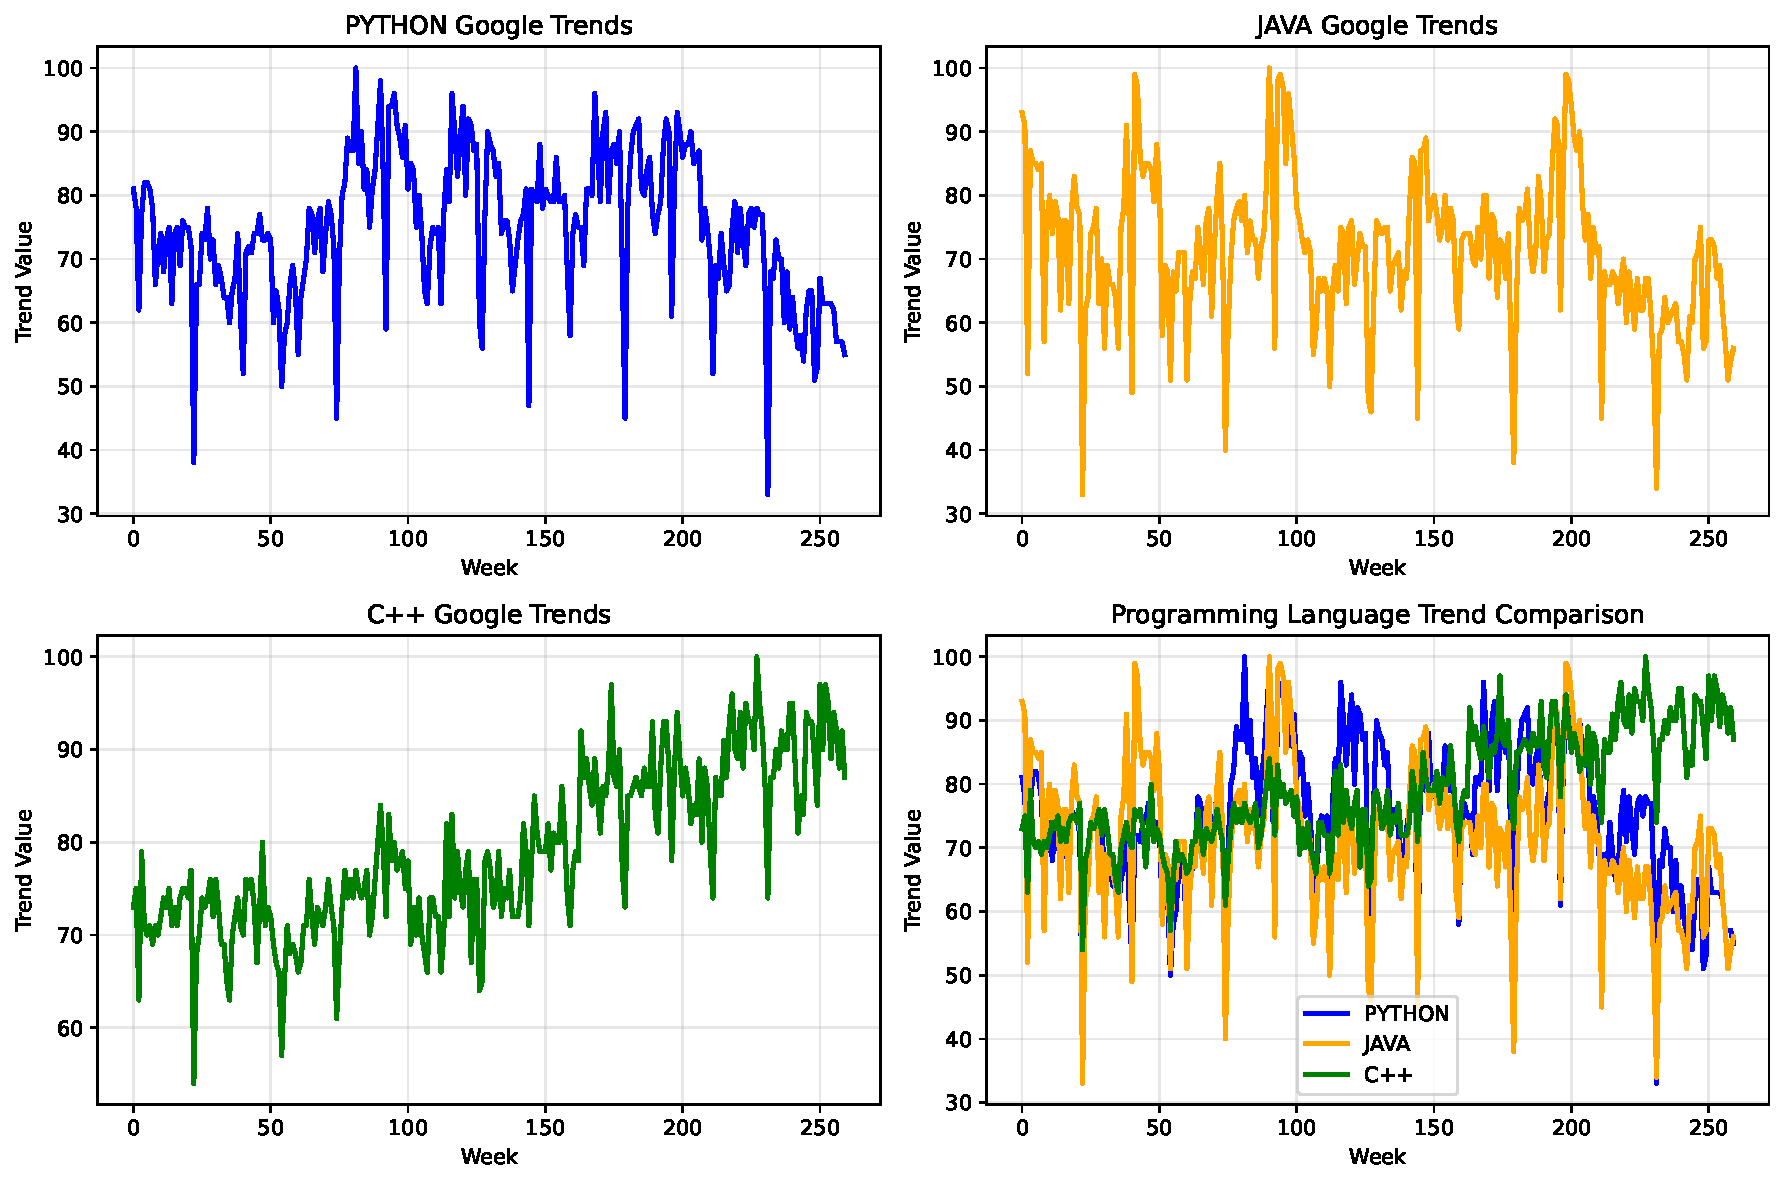
\includegraphics[width=0.9\textwidth]{figures/fig7_multilang_trends.pdf}
\caption{プログラミング言語トレンド比較(Python, Java, C++)}
\label{fig:multilang-trends}
\end{figure}

\subsection{解析手法}

\subsubsection{データ統合アプローチ}

各言語の時系列データ $\mathbf{X}_{\text{python}}$, $\mathbf{X}_{\text{java}}$, $\mathbf{X}_{\text{c++}}$ に対して、以下の手順でSVD解析を実施した:

\begin{enumerate}
  \item 各時系列を同一ウィンドウサイズ $w=12$ でdelay coordinates行列に変換
  \item 得られた行列を縦方向に連結して統合行列 $\mathbf{X}_{\text{stack}}$ を作成
  \item 統合行列に対してSVDを適用し、上位 $k=3$ 成分を抽出
\end{enumerate}

統合行列のサイズは $(63 \times 12)$ となり、これは3言語の時間窓(各21個)を縦方向に積み重ねた結果である。

\subsection{主要な発見}

\subsubsection{特異値と寄与率}

図\ref{fig:multilang-singular-values}に示すように、SVD解析により得られた上位3成分の特異値は以下の通りであった:
\begin{equation}
[\sigma_1, \sigma_2, \sigma_3] = [2076.26, 115.32, 93.64]
\end{equation}

特に注目すべきは、第1成分の寄与率が99.5\%と圧倒的に高いことである。これは、3つのプログラミング言語のトレンドに極めて強い共通パターンが存在することを示している。

\begin{figure}[H]
\centering
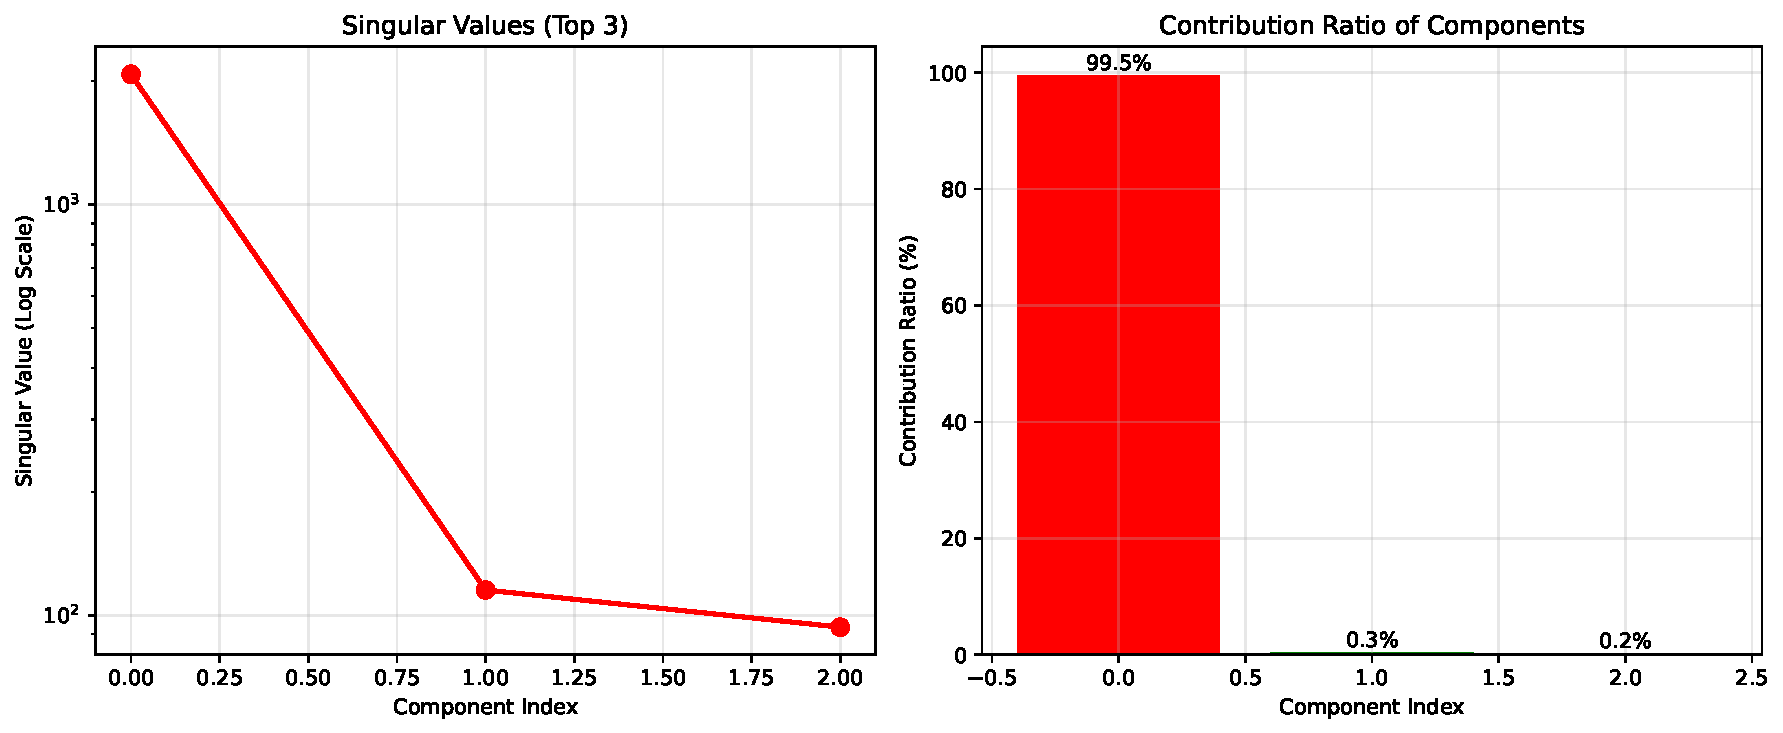
\includegraphics[width=0.9\textwidth]{figures/fig8_multilang_singular_values.pdf}
\caption{特異値と寄与率(多次元SVD解析)}
\label{fig:multilang-singular-values}
\end{figure}

\subsubsection{局所パターンの解析}

図\ref{fig:multilang-vh-patterns}は、各成分のVh局所パターンを示している。これらのパターンは、12週間の時間窓内での微細な変動構造を表現している。

\begin{figure}[H]
\centering
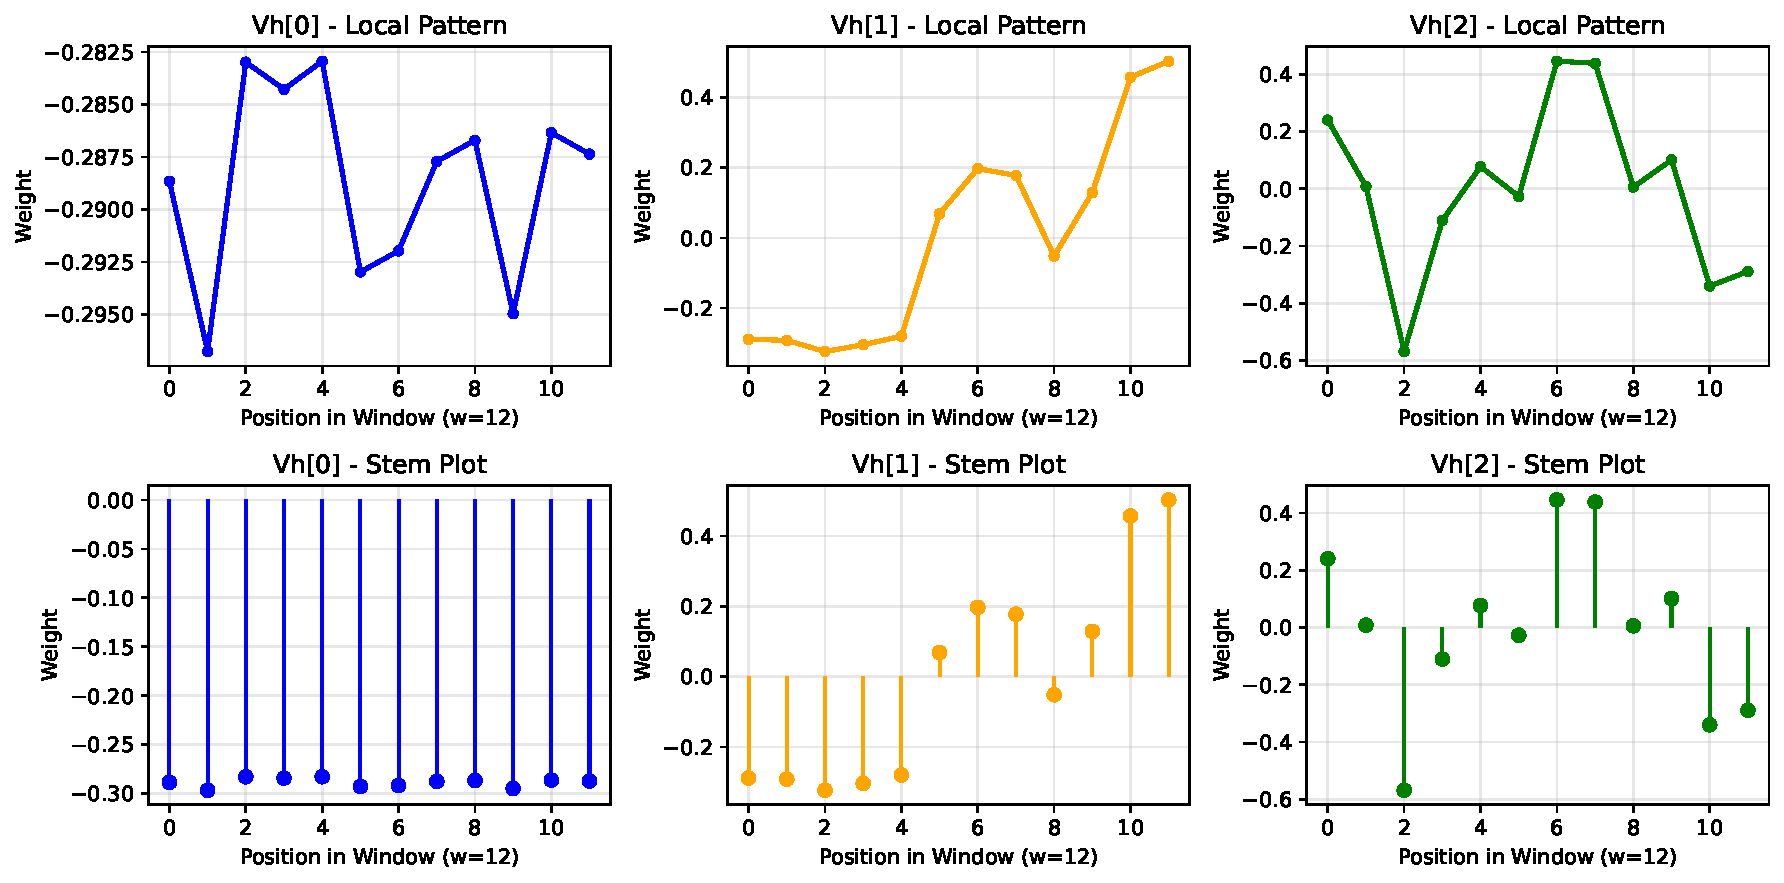
\includegraphics[width=0.9\textwidth]{figures/fig9_multilang_vh_patterns.pdf}
\caption{多次元SVDにおけるVh局所パターン}
\label{fig:multilang-vh-patterns}
\end{figure}

\subsubsection{言語間の相関構造}

図\ref{fig:multilang-correlation}は、言語間の相関分析結果を示している。言語間の相関分析では、以下の重要な知見が得られた:

\begin{itemize}
  \item Python-Java間が最も高い相関(相関係数:0.524)を示した
  \item 3言語とも第1成分に強く寄与しており、技術トレンドの共通基盤を形成
  \item 各言語固有の変動パターンは第2, 3成分に反映
\end{itemize}

\begin{figure}[H]
\centering
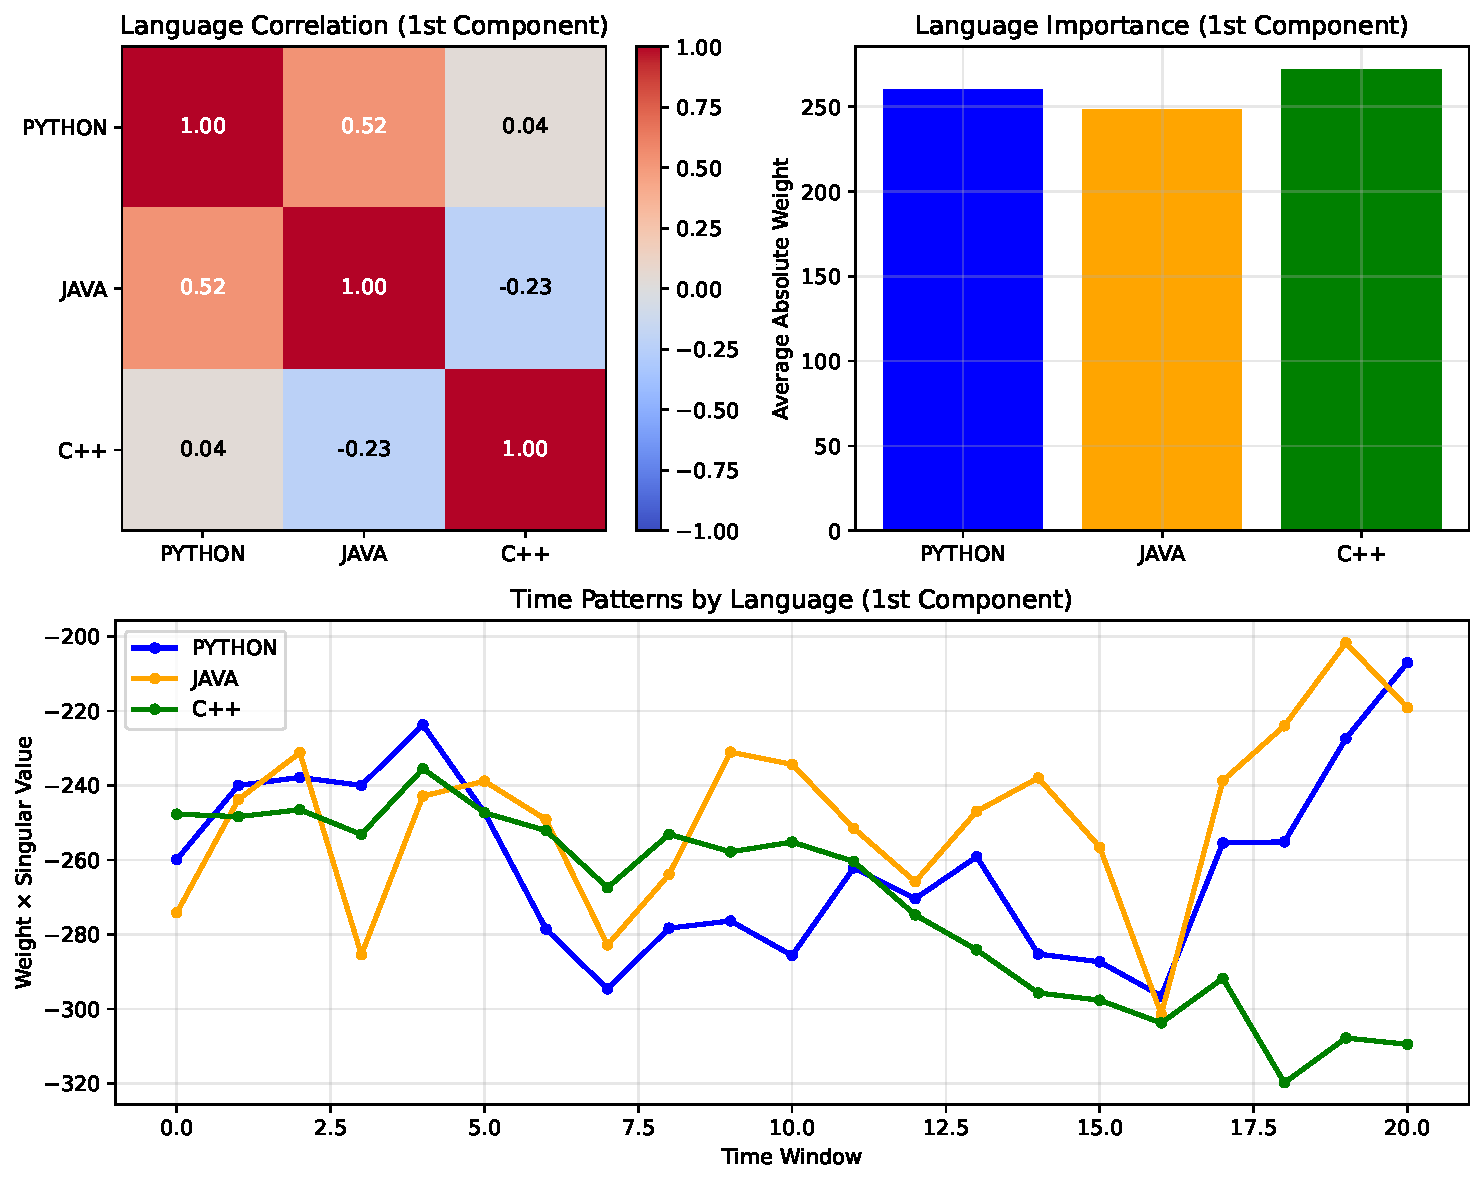
\includegraphics[width=0.9\textwidth]{figures/fig10_multilang_correlation.pdf}
\caption{言語間相関分析と時間パターン比較}
\label{fig:multilang-correlation}
\end{figure}

\subsection{考察}

\subsubsection{共通パターンの意味}

第1成分の極めて高い寄与率(99.5\%)は、プログラミング言語の人気度変動に強い共通基盤が存在することを示唆している。これは以下の要因によると考えられる:

\begin{itemize}
  \item 技術トレンド全体の周期性(年間サイクル)
  \item プログラミング学習需要の共通変動
  \item 産業界全体のテクノロジー採用パターン
\end{itemize}

\subsubsection{言語間の類似性と差異}

Python-Java間の高い相関(0.524)は、これらの言語が:
\begin{itemize}
  \item 汎用プログラミング言語としての共通の用途
  \item 教育・学習環境での普及
  \item エンタープライズでの広範な採用
\end{itemize}
という特徴を共有していることを反映していると解釈できる。

\subsection{結論と展望}

本解析を通じて、SVDが多次元時系列データの統合解析に極めて有効であることが実証された。特に:

\begin{itemize}
  \item 複数時系列の共通パターン抽出に成功
  \item 定量的な類似性評価手法の確立
  \item 効率的な次元削減と特徴表現の実現
\end{itemize}

今後の発展として、以下のような方向性が考えられる:

\begin{itemize}
  \item より多くのプログラミング言語への適用
  \item 異なる時間スケールでの解析(月次、年次など)
  \item 地域別トレンドの比較分析
  \item 他の技術キーワードとの関連性調査
\end{itemize}

\section{課題4-1:Multi-Scale Basis (MSB) 論文のまとめ}

本節では、SVDを用いた時系列解析の理論的背景として重要な論文 ``Multi-Scale Basis (MSB) for Time Series Data Mining'' の内容をまとめる。

\subsection{問題設定と背景}

大規模時系列ストリームデータにおけるパターン抽出において、従来手法では以下の課題が存在していた:

\begin{itemize}
  \item スケール(時間幅)の選択に一貫性がない
  \item 異なるスケールにまたがるパターンが見逃される可能性がある
  \item 効率的なパターン抽出手法の必要性
\end{itemize}

\subsection{Multi-Scale Basis (MSB) の提案}

著者らは、複数の時間スケールにわたる重要な部分パターン(basis)を効率的に抽出する手法を提案している。主なアプローチは以下の通り:

\begin{enumerate}
  \item ストリームデータをスライディングウィンドウで分割
  \item 各ウィンドウを異なる長さ(スケール)で表現
  \item 各スケールで局所的なパターンを抽出(SVDなどを使用)
  \item 抽出された部分パターンから、冗長性が少なく情報量の高いものを選択
  \item これらを組み合わせて多スケール基底(MSB)を形成
\end{enumerate}

この基底により、任意の入力時系列を効率的に近似・表現することが可能となる。

\subsection{Power Profile の導入}

MSBの重要な特徴として、各スケール(時間幅)ごとの情報量を測る「Power Profile」という概念を導入している:

\begin{itemize}
  \item ある時間幅 $w$ に対し、最も重要な部分パターン(ベクトル)の情報寄与を定量化
  \item これにより、どのスケールが最も有益な構造を含むかを客観的に判断可能
  \item スケール選択の定量的な指標として機能
\end{itemize}

\subsection{実験による検証}

論文では以下のデータセットを用いて手法の有効性を検証している:

\begin{itemize}
  \item 人工的に生成したシグナル
  \item 実際の株価データ
  \item Google Trendsデータ
\end{itemize}

主な評価内容:

\begin{itemize}
  \item MSBの表現力(元信号との近似誤差)
  \item 従来手法(DCT、Waveletなど)との比較
  \item Power Profileによるスケール選択の有効性
\end{itemize}

実験結果として、以下の知見が得られている:

\begin{itemize}
  \item MSBは他の手法と比較して高精度な近似を実現
  \item Power Profileを用いることで、最適な時間幅の自動選択が可能
  \item 少数のベクトル(basis)のみで高精度の再構成が可能
\end{itemize}

\subsection{本研究との関連}

本研究で実施した花粉症データおよびプログラミング言語トレンドデータの解析は、MSB論文で提案された考え方と以下の点で関連している:

\begin{itemize}
  \item 複数の時間スケール($w=12$、$w=24$)での解析を実施
  \item SVDを用いた局所パターンの抽出
  \item 再構成誤差による定量的評価
\end{itemize}

MSB論文の知見は、より複雑な時系列データ解析への応用可能性を示唆しており、今後の研究の方向性を考える上で重要な示唆を与えている。

\end{document}
